% --------------------------------------------------------------------- %
% Modelo adaptado pelo aluno voluntário João Antonio Teixeira Sucupira  %
% Supervisão do Prof. Daniel Fernando Pigatto                           %
% Programa de Pós-graduação em Computação Aplicada (PPGCA)              %
% Universidade Tecnológica Federal do Paraná (UTFPR)                    %
% --------------------------------------------------------------------- %

\documentclass{if-beamer}
\usepackage{minted}
\usepackage{svg}
\renewcommand\MintedPygmentize{"/Users/yinshi/Library/Python/3.9/bin/pygmentize"}
% --------------------------------------------------- %
%                  Presentation info	              %
% --------------------------------------------------- %
\title[Dissecting the moat regime at low energies I]{\huge \textbf{Dissecting the moat regime at low energies I: Renormalization and the phase structure}}
%\subtitle{Universidade Tecnológica Federal do Paraná}
\author[Shi Yin]{\huge \negrito{Shi Yin}}
\institute[JLU]{
    \large \textit{Justus-Liebig-Universität Gießen} \\
    \textit{Institut für Theoretische Physik}
}
\date{08.10.2025, Dalian}
%\logo{
%\hspace{0.2cm}
%
\includegraphics[scale=.03, clip]{figuras/fQCDLogoFR.png}\hspace{0.2cm}
%
\includegraphics[scale=.6, clip]{figuras/jlu-logo-600.png}\hspace{0.2cm}
%
\includegraphics[scale=.23, clip]{figuras/imgpsh_fullsize_anim.jpg}\hspace{0.2cm}
%\includesvg[height=40pt]{figuras/CRC-TR211long.svg}
%}
\titlegraphic{  \begin{tabular}{cccc}
\hspace{-1.cm}

\includegraphics[scale=.03, clip]{figuras/fQCDLogoFR.png}&

\includegraphics[scale=.6, clip]{figuras/jlu-logo-600.png}&

\includegraphics[scale=.2, clip]{figuras/imgpsh_fullsize_anim.jpg}&
\includesvg[height=40pt]{figuras/CRC-TR211long.svg}
  \end{tabular}}
\subject{Presentation subject} % metadata
%trim={<left> <lower> <right> <upper>}
\graphicspath{{figuras/}}
% --------------------------------------------------- %
%                    Title + Schedule                 %
% --------------------------------------------------- %

\begin{document}

\begin{frame}
  \titlepage
\end{frame}

\begin{frame}{Outline}
  \tableofcontents
\end{frame}

% --------------------------------------------------- %
%                      Presentation                   %
% --------------------------------------------------- %

%%%%%%%%%%%%%%%%%%%%%%%%%%%%%%%%%%%%%%%%%%%%%%%%%%%%%%%%%%%%%

\section{Introduction}

\subsection{QCD phase diagram}
\begin{frame}{QCD phase diagram}

        %\begin{columns}
        %\begin{column}{0.43\textwidth}
        %    \vspace{-7cm}
        %    \begin{itemize}
        %    \item Lattice QCD (at vanishing chemical potential)\\~\
        %    \item Dyson-Schwinger Equations (DSE)\\~\
        %    \item Functional renormalization group (fRG)\\~\
        %    \item ...
        %    \end{itemize}
        %\end{column}
        %\begin{column}{1\textwidth}
            \centering{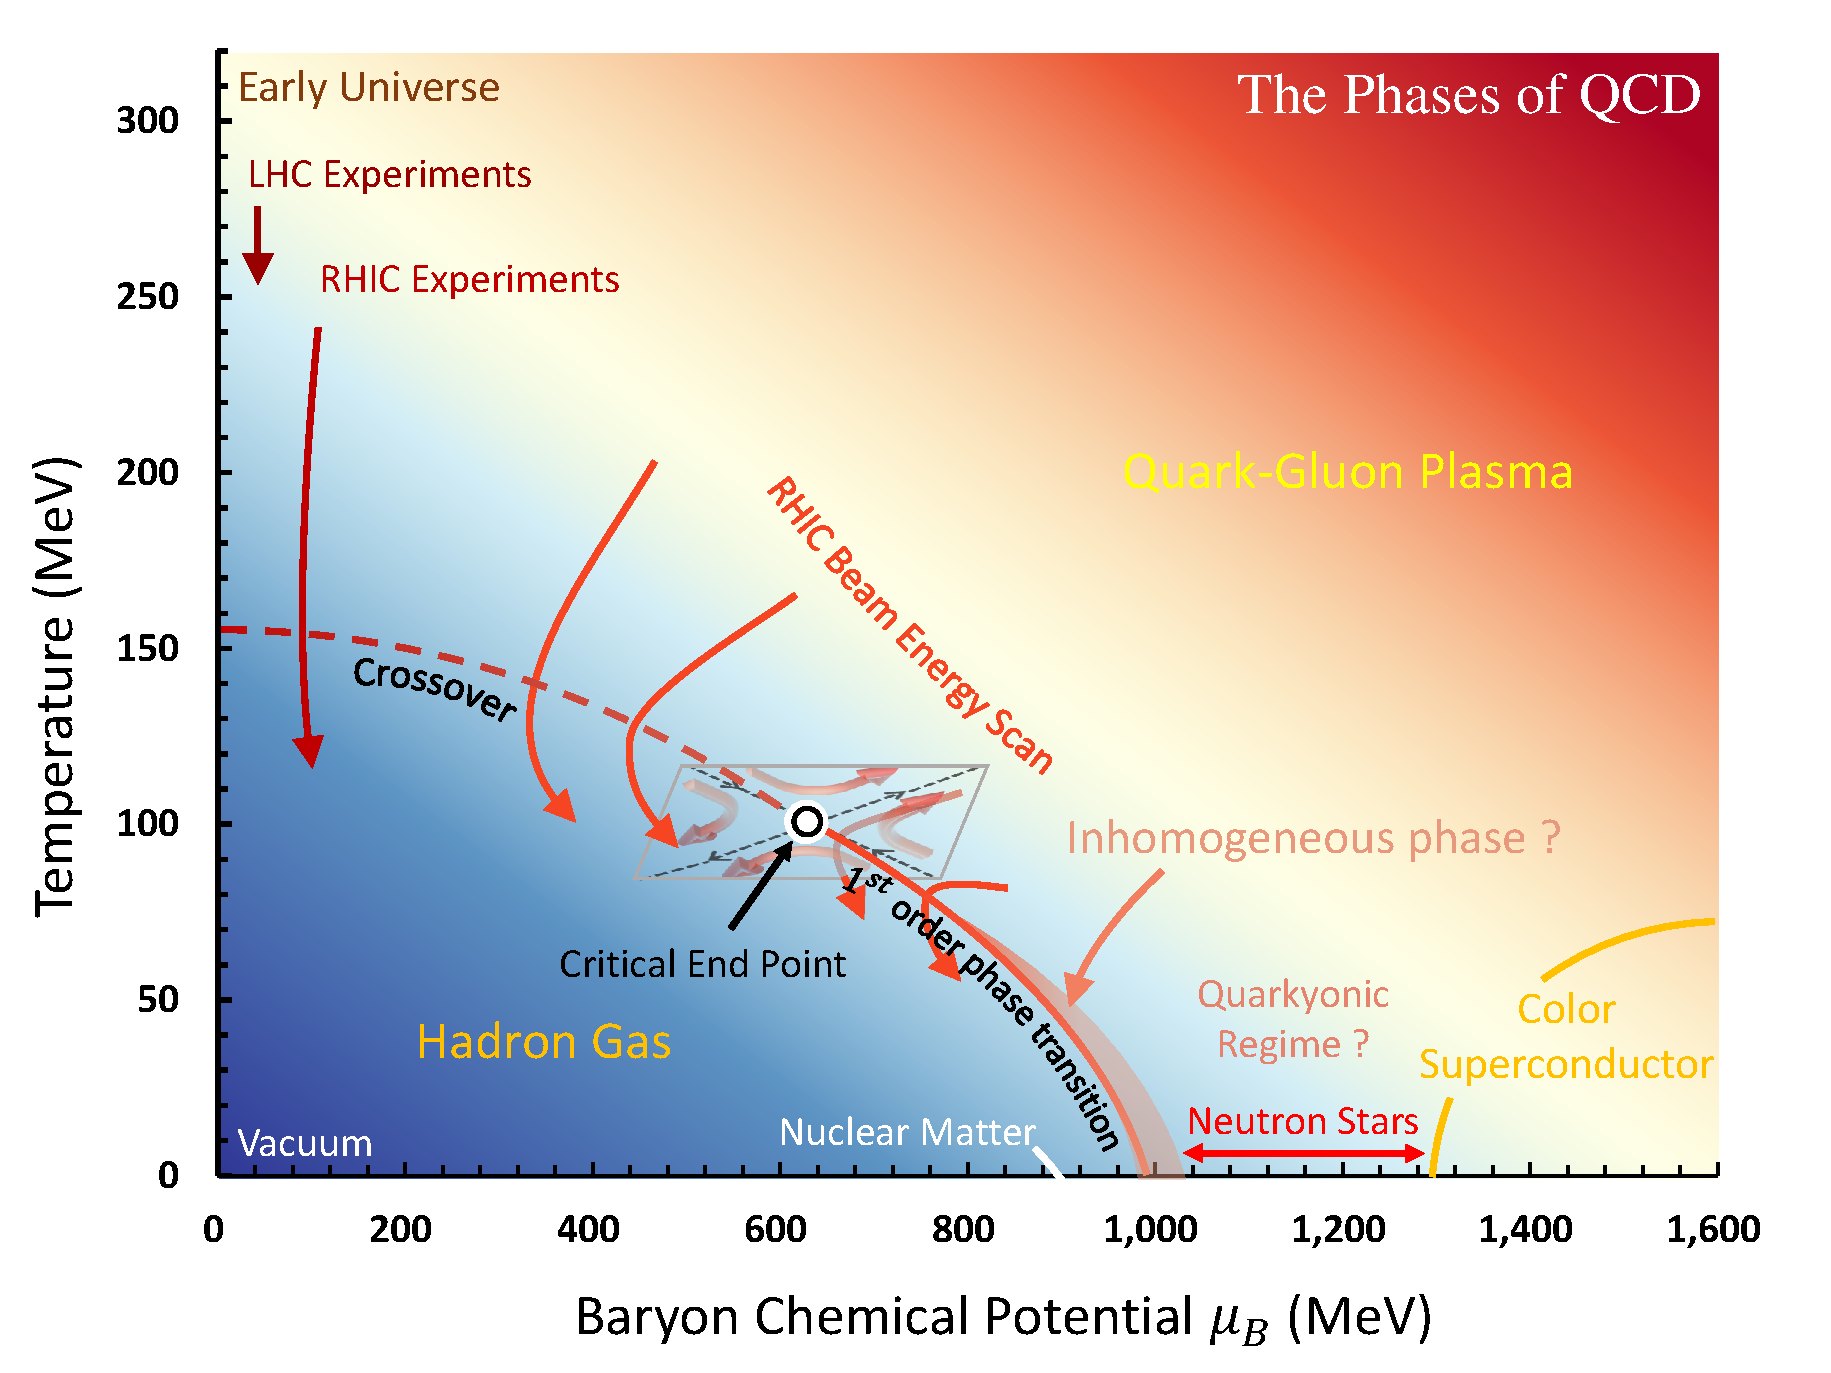
\includegraphics[width=0.87\linewidth]{figuras/chap1_phase20240311.pdf}}\\~\
            \centering{\color{blue}{SY, Tan, Fu (2023)}}
        %\end{column}
        %\end{columns}
    %\begin{itemize}
    %    \item Item 1
    %    \item Item 2
    %    \item Item 3
    %\end{itemize}

\end{frame}

\subsection{Experimental data}
\begin{frame}{Experimental data}

    Texto com a motivação do trabalho.

\end{frame}

\subsection{Theoretical predictions}
\begin{frame}{Predictions from functional methods}

    Texto com a motivação do trabalho.

\end{frame}

%%%%%%%%%%%%%%%%%%%%%%%%%%%%%%%%%%%%%%%%%%%%%%%%%%%%%%%%%%%%%

\section{Metodologia}

\begin{frame}{Métodos de desenvolvimento}

    Texto que apresenta a metodologia.

\end{frame}

%%%%%%%%%%%%%%%%%%%%%%%%%%%%%%%%%%%%%%%%%%%%%%%%%%%%%%%%%%%%%

\section{Resultados}

\begin{frame}{Resultados}

\begin{itemize}
    \item Resultados 1
    \item Resultados 2
\end{itemize}

\begin{block}{Bloco de destaque}
    \begin{itemize}
        \item Item 1
        \item Item 2
        \item Item 3
        \item Item 3
    \end{itemize}
\end{block}

\end{frame}

%%%%%%%%%%%%%%%%%%%%%%%%%%%%%%%%%%%%%%%%%%%%%%%%%%%%%%%%%%%%%

\end{document}
